\documentclass{article}
% \usepackage[utf8]{inputenc}
% \usepackage[english,swedish,german]{babel}
\usepackage{graphicx} % Required for inserting images

\title{FlexBatt: Power Electronics for Flexible and Sustainable Batteries}
\author{Arvind Balachandran, Tomas Jonsson, and Lars Eriksson}
\date{August 2023}

\usepackage{hyperref}
\hypersetup{
    colorlinks   = true, %Colours links instead of ugly boxes
    urlcolor     = blue, %Colour for external hyperlinks
    linkcolor    = black, %Colour of internal links
    citecolor   = black %Colour of citations
    }

% \usepackage{biblatex}
% \addbibresource{references.bib}

\begin{document}

\maketitle

\begin{figure}[!b]
    \centering
    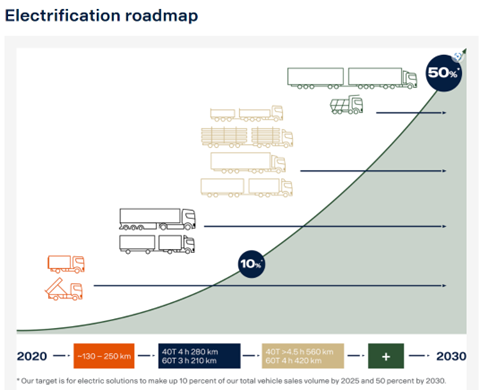
\includegraphics[width=0.8\textwidth]{Figures/EV_sales.png}
    \caption{Scanias roadmap for electrifying the commercial vehicle fleet.}
    \label{fig:EVsales}
\end{figure}
\section{Background}
Road freight transportation is the backbone of trade and commerce in the European Continent, and heavy-duty vehicles (HDVs) carry about 71.3\% of the freight transport over land \cite{aceatrucks}. Moreover, about 98\% of the HDV fleet is powered by diesel, contributing to about 25\% of the EU automotive greenhouse-gas emissions \cite{ccesregulation}. As part of the effort to reduce greenhouse gas emissions, intergovernmental organizations, such as the European Commission, have introduced stricter legislation standards to reduce the negative impact of the automotive sector on climate and the environment by ensuring zero-emission mobility within the next few years \cite{european2011communication}. As a result, several leading heavy-duty vehicle manufacturers, such as Scania CV AB, have announced plans to transition to 100\% electric heavy-duty vehicle sales by 2040 \cite{ragon2021co2}. In collaboration with Scania CV AB and SEM AB, this project aims to demonstrate, develop, and contribute to making society's road freight transportation efficient, durable, cost-effective, and fossil-free.
\begin{figure}[!t]
    \centering
    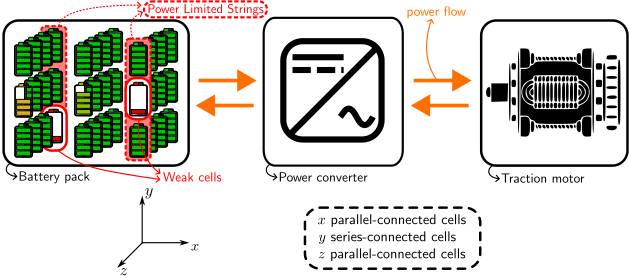
\includegraphics[width=\textwidth]{Figures/conventional_powertrain.png}
    \caption{Conventional electric vehicle powertrain with a large battery pack containing weak cells shown in red.}
    \label{fig:convEVpoertrain}
\end{figure}
\begin{figure}[!b]
    \centering
    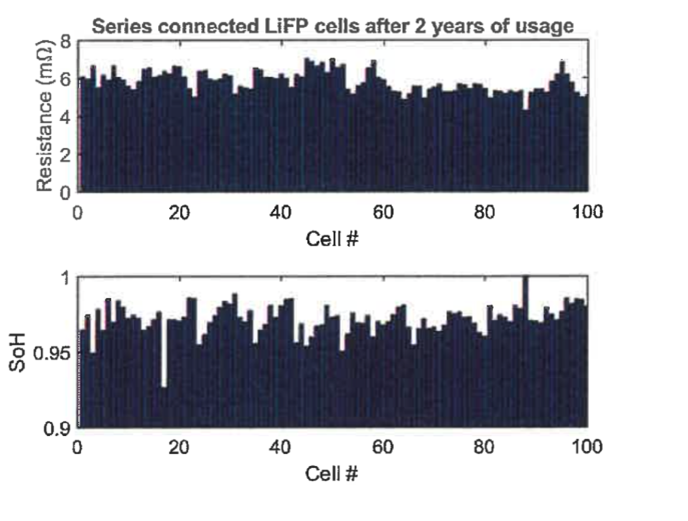
\includegraphics[width=0.8\textwidth]{Figures/SOC_IR_dist.png}
    \caption{ Internal resistance and state-of-health (SOH) for 100 series connected cells after two years of use.}
    \label{fig:IR_SOC_dist}
\end{figure}

A significant challenge the automotive industry faces in transitioning to electrification and, thus, to a sustainable society is the cost and lifespan of battery packs in electric vehicles. The battery pack's state of health (SOH) is a critical parameter determining the battery's end-of-life and is often determined by the weakest cell in the pack. When the SOH of the battery pack falls below 80\% (often the SOH of the weakest cell), the battery pack is considered at the end of life and should be replaced. This results in additional expenses for the consumer and creates an extra environmental burden \cite{canals2022electric}. To understand this problem in detail, consider a conventional electric vehicle with a large battery pack with several thousand hard-wired series- and parallel-connected cells (Figure~\ref{fig:convEVpoertrain}). Due to variations in the manufacturing of the cells and several other factors, the distribution of voltages and the state of charge among the cells are non-homogeneous and vary during operation \cite{schuster2015lithium} and in Figure~\ref{fig:IR_SOC_dist}, the internal resistance and state of health (SOH) for 100 series connected cells in a battery pack after two years of use is shown.
\begin{figure}[!b]
    \centering
    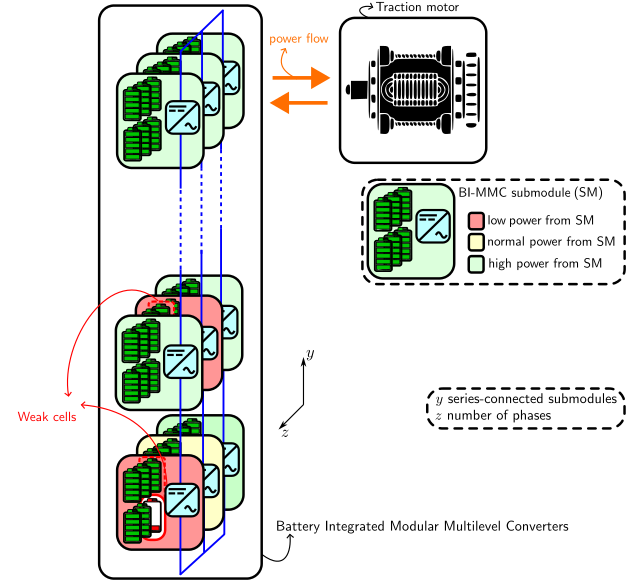
\includegraphics[width=\textwidth]{Figures/BI_MMC_powertrain.png}
    \caption{Battery-integrated modular multilevel converter (BI-MMC) based battery electric vehicle powertrain with a BI-MMC with small battery packs in submodules and a traction motor.}
    \label{fig:BIMMCpoertrain}
\end{figure}
From the figure, the relative difference in the SOH between the healthiest and the weakest cell in the pack is about 8\%. More concerningly, the internal resistance of the weakest cell is almost two times greater than the healthiest, resulting in non-uniform heat distribution, leading to the formation of hotspots and overheating, thus limiting both the power and energy the pack can deliver. Furthermore, every cell has a minimum and maximum voltage limit, and these limits must be maintained to prevent the battery from being destroyed \cite{garche2018electrochemical}. The weak cells (shown in red in Figure~\ref{fig:convEVpoertrain}) reach this limit faster than others, and even if a single cell in the pack reaches the limit, the pack cannot be used, rendering the entire pack useless.

The project aims to develop a system that enables individual cell control, thereby improving the battery pack's robustness, lifetime, and energy utilization. The selected approach for achieving individual cell control is by using battery-integrated modular multilevel converters (BI-MMC). BI-MMCs have several cascaded stages of bi-directional DC to AC converters called submodules (SM) as shown in Figure~\ref{fig:BIMMCpoertrain}. Each submodule consists of a few series- and parallel-connected cells. BI-MMCs can actively react to the driving scenario and redirect the energy flow among submodules and, in extreme cases, disconnect weak cells from the pack, thereby improving the energy efficiency, safety, and lifetime of the electric vehicles.

\section{State-of-the-art}
Modular multilevel power electronic converters, established in the early 2000s, have yet to be extensively explored in electric vehicles with modular battery packs. This emerging approach has the potential to enhance electric vehicle efficiency and longevity. This section covers industry advancements, ongoing university research, and previous project contributions, setting the stage for future research directions.
% Modular multilevel power electronic converters have existed since the early 2000s, but their application in electric vehicles with modular battery packs remains relatively unexplored. The concept of using battery-based modular multilevel converters is an emerging domain with significant potential for enhancing the efficiency and longevity of electric vehicles. The first subsection presents the state-of-the-art in the industry followed by the current research in the Universities and finally the contributions and continuations from the previous project

\subsection{Industrial trends}
In the past couple of years, the industry has witnessed an increase in the adoption of BI-MMC-based solutions. Notably, three out of the four companies listed below were founded in 2022 and have promised improvements in efficiency and longevity.    

The Intelligent Battery Integrated System (IBIS) is a collaborative research project between Stellantis and Saft. This demonstrator has been operational since the summer of 2022 \cite{ChargedEVs}. Currently, the IBIS project team is directing its efforts towards constructing a fully functional prototype vehicle and there are plans to integrate this technology into Stellantis vehicles by the end of this decade. 

In collaboration with Kempten-based start-up BAVERTIS, ABT e-line develops an innovative alternative driveline employing multilevel technology \cite{ABTSportsline}. BAVERTIS specializes in developing battery modules, spanning voltage ranges from 3.6 V to 300 V AC or DC. With the incorporation of additional modules, the objective is to attain a driveline voltage of 1000 V. The alternative driveline promises higher performance, increased safety, and increased reliability. ABT e-line's partnership with Volkswagen Commercial Vehicles further extends to the production of electrified versions of the Caddy and Transporter \cite{ABTeline}. 

TAE Power Solutions develops two technologies: Intelligent AC power (ACi) and Converter Battery Module (CBM). These technologies integrate energy storage and power electronics, facilitating rapid charging, optimizing performance, extending travel range, and enhancing battery longevity for both electric mobility and stationary applications \cite{TAETech}. TAE Power Solutions collaborates alongside BMW and other partners to jointly develop advanced battery systems.

Brill Power, a spin-out enterprise from Oxford University, has a scalable solution tailored for extensive large-scale energy storage applications \cite{BrillPower}. Their latest modular system, BESA BP6X1, combines battery management, power conversion, edge computing, monitoring, and analytics in one fully integrated solution. This comprehensive integration has optimal battery performance. Brill Power wants to expand the utilization of its modular system into commercial vehicles.

This project focuses on optimizing the entire powertrain, reducing the number of sequential power conversion stages, thus further improving the battery lifetime, lifetime cost, thermal management, and faster charge rates focusing on heavy-duty commercial vehicles.

\subsection{Current research}
The charging time for electric vehicles is significantly longer than the refueling time for conventional vehicles. To achieve a short charging time, efficient DC fast chargers capable of delivering high power are required. To meet the changing needs of medium- and heavy-duty commercial vehicles, megawatt charging systems are under development \cite{meintz2022charging}. An advantage of BI-MMCs is that the requirement for an onboard charger for AC charging, necessary for conventional electric vehicle powertrain, becomes obsolete \cite{buberger2021charging}. However, DC charging is more challenging since the battery charging power flows through the submodules. Our previous research work on DC charging capabilities of different BI-MMC architectures \cite{balachandran2023dc} showed that a maximum power of 3\,MW is achieved. BI-MMCs, with their submodules, can enable pulsed charging and several pieces of research indicate improved battery lifetime, up to 80\% improvement in lifetime, with pulsed charging \cite{huang2020review,huang2021effects}. The goals of this research project are to understand the trade-offs between charging time, increased lifetime, and converter rating for pulsed charging using BI-MMCs and demonstrate the pulsed charging capabilities of BI-MMCs.

Another pivotal element within the electric vehicle powertrain is the electric machine, which not only carries a significant cost but also holds substantial volume importance. Electric machines have been used in industrial applications for nearly a century. While controlling the electric machine around the rated power is straightforward, extracting the maximum performance presents a significant challenge. This is overcome by introducing power electronic converter-based electric machine drives and all electric vehicles have it. The conventional electric vehicle powertrain uses a 2-level inverter (shown in Figure ~\ref{fig:convEVpoertrain}) and these converters have high-voltage switching steps (voltage steps of 600 to 1000\,V) that may cause high stresses of bearings. If mitigation measures are not taken, electric machines can fail \cite{bell2001experience}, and replacing the electric machine can get expensive. 

To overcome these challenges, the following countermeasures are considered during the design phase:
\begin{enumerate}
    \item Increased conduction insulation, which increases the size and weight of the electric machine.
    \item Decoupling the electrostatic fields from the rotor by shielding also increases the electric machine's size and weight.
    \item Adding filters and chokes, which increases the cost of the electric vehicle powertrain.
    \item Reducing the $dv/dt$ switching effects at the drive by minimizing drive input voltages, increasing the power converter losses. 
\end{enumerate}
Harmonic distortion is the degree to which undesirable harmonics are created during power conversion. The higher the harmonic distortion, the higher the losses in the electric machine. The 2-level inverter in conventional electric vehicle powertrains has high harmonic distortion, resulting in increased losses in the electric machine. 

The design and control of a BI-MMC architecture with active balancing strategies are presented in \cite{quraan2015design} and claimed an increase in lifetime compared to a conventional electric vehicle powertrain due to the inherent balancing between the cells. However, the paper considered half-bridge converters as submodules, this increases losses on the battery.
\cite{josefsson2015investigation} explored the concept of BI-MMCs with full-bridger submodules, or cascaded H-bridge inverters (CHB), for passenger cars and experimentally showed higher efficiencies compared to the conventional 2-level inverter. Several other BI-MMC architectures, such as modular multilevel series-parallel converters (MMSP) were investigated in \cite{korte2017efficiency,kersten2021modular} and showed improvements in efficiency. Technical University of Kaiserslautern and Universität der Bundeswehr München, are looking into battery modular multilevel management (BM3) converters (similar to BI-MMCs) and have shown improved efficiency compared to conventional 2-level inverter \cite{kuder2020battery}. \cite{ma2018analysis} showed that BI-MMCs have improved fault ride-through capabilities, potentially increasing both the reliability and lifetime of powertrains with BI-MMCs.

\subsection{BattVolt Project}
The previous project led to a Licentiate thesis \cite{balachandran2023battery} that included the following contributions:
\begin{enumerate}
    \item The design and evaluation of 3-phase and 6-phase BI-MMC architectures; comparisons are made against a conventional 2-level inverter for a 40-ton 400 kW commercial vehicle. The evaluation considers the total number of submodules, energy rating of the DC-link capacitors, battery losses, capacitor losses, and semiconductor losses. The evaluation showed that the BI-MMCs have lower semiconductor losses than the conventional 2-level inverter. However, the BI-MMCs have higher capacitor and battery losses. 
    \item The impact that the number of series connected cells per submodule has on the total losses of the BI-MMC. The study showed that 5- to 6-series connected cells have the lowest losses. 
    \item The design principles for optimization of the DC-link capacitors and the MOSFET switching frequency; are supported by experimental validation for the loss distribution within a submodule. 
\end{enumerate}
As a continuation, in this project, the losses in the BI-MMCs can be further reduced with the nearest level control technique. 
\begin{enumerate}
    \item[4.] The fourth contribution is a methodology for determining the battery impedance using the full-load converter current. 
\end{enumerate}
As a continuation, this project aims to compare battery losses in BI-MMCs using impedance spectroscopy and heat measurements using a calorimeter. 
\begin{enumerate}
    \item[5.] In a conventional battery pack, the battery is connected directly to the fast charger's DC supply. However, in a BI-MMC, the battery and the inverter are integrated, potentially increasing the DC charging capabilities because higher voltages can be achieved during charging than during operation. The fifth contribution is thus the derivation and investigation of the maximum DC charging power of BI-MMCs assuming the same submodule semiconductor losses during traction. The analysis showed that most BI-MMCs have a maximum DC charging power of about 1MW.
\end{enumerate}
As a continuation, in this project, the analysis is being extended to pulsed charging, followed by an experimental implementation. 

\section{Potential}
Examining the electric vehicle powertrain, it becomes clear that the battery constitutes the highest cost and is the key limiting factor for the electric vehicle's lifespan.
The clear research focus is on strategies to minimize costs, enhance efficiency, and increase the lifetime.
Since BI-MMCs have several cascaded stages of bi-directional DC to AC converters, called submodules as shown in Figure~\ref{fig:BIMMCpoertrain}, and each submodule consists of a few series- and parallel-connected cells, the energy exchange between submodules can be dynamically adjusted in response to driving conditions, i.e., energy exchange between the cells in a battery pack can be dynamically adjusted in response to driving conditions. Furthermore, in extreme cases, submodules with weak cells can be disconnected entirely. This relieves the stress on the weak cells thus improving the lifetime and more importantly, the safety of electric vehicle batteries. Since the weak cells can now be controlled separately, the state of health of the pack is no longer equal to the state of health of the weakest cell, but rather the average state of health of the entire pack. Thus, the lifetime of the battery pack can be increased and in turn, decreases the total cost of ownership. Quantitatively, the BI-MMC architecture can potentially extend the lifetime of the batteries by 71\% compared to a conventional electric vehicle battery pack \cite{skegro2023analysis}. This almost doubling of the battery pack's lifespan could lead to reduced electric vehicle total ownership costs and an extended lifetime.

The charging time for electric vehicles is significantly longer than the refueling time for conventional vehicles. To achieve a short charging time, efficient DC fast chargers capable of delivering high power are required. As megawatt chargers proliferate and pulsed charging potentially extends battery life by up to 80\%, the potential of BI-MMCs to transform charging and refueling infrastructure becomes increasingly evident. This can further improve the lifetime of the battery pack and, in turn, the increased lifetime of the electric vehicle.

Another pivotal element within the electric vehicle powertrain is the electric machine, which not only carries a significant cost but also holds substantial volume importance. 
A drawback of the conventional electric vehicle powertrain with a 2-level converter is the elevated mechanical stresses on the bearings within the electric machine. This leads to the oversizing of the electric machine, consequently causing a proportional increase in its volume. Furthermore, another drawback of the conventional electric vehicle powertrain is the high harmonic distortion from the 2-level inverter. This causes an increase in the losses and substantially decreases the efficiency of the electric machine, which in turn, reduces the efficiency entire electric vehicle powertrain. BI-MMCs have considerably lower harmonic distortion potentially reducing the losses and substantially increasing the efficiency of the electric machine. Furthermore, the low-voltage switching steps (voltage steps of 5 to 60\,V) potentially reduce the electric machine size, insulation, and core losses. This, in turn, increases the overall efficiency of the electric vehicle powertrain. Furthermore, BI-MMCs can potentially increase the robustness of the electric machine thereby reducing the cost of the electric machine.

The third important component in the electric vehicle powertrain is the power electronic converter. The conventional electric vehicle powertrain for commercial vehicles typically has a 2-level inverter.  Our previous research project \cite{balachandran2023battery} showed that such an inverter has an efficiency of 99\% at average power, which corresponds to about 900\,W of power loss. Moreover, our previous research project \cite{balachandran2023battery} on the evaluation of different BI-MMC architectures shows that most have higher efficiency, some reaching up to 99.4\% at average power. This translates to about 600\,W of power loss, nearly halving the losses and extending the electric vehicle's driving range. Our previous research work \cite{balachandran2023battery} considered a high-frequency pulse width modulation control technique for BI-MMCs, but in this research work, alternative control techniques are explored to reach the efficiencies of about 99.6\%. This translates to about 400\,W of power loss, further extending the electric vehicle's driving range. 

The results from the research project will be published in several international journals and conferences, thus enabling international contributions and collaborations. 

Swedish industries such as Scania CV AB and SEM AB support the experimental buildup by manufacturing the prototypes of the hardware components for the project. Furthermore, the core project team is supported by Scania and SEM resources, and with engagement in the project, they can take the results into the organization, continue the technology development to higher TRL levels, and start the integration in their product development.

\nocite{the_icct_why_2021}
\nocite{sveriges_miljomal_utslapp_nodate}
\nocite{fossilfrittsverige}

\bibliographystyle{apalike}
\bibliography{references,batteryRefs,other}

% \printbibliography

\end{document}
